\subsection{Required Laser Power} 
\label{ssec:resolution}
The requirement for the altimetry mode changes based on the height. The target is a resolution of at least $0.1\,\%$. To ensure that this requirement is met, both the largest altitude of $8\,km$, and the smallest altitude of $500\,m$ will be investigated.

The minimum resolution for the largest and shortest altitude are $8\,m$ and $0.5\,m$ respectively. The maximum allowable FWHM can be calculated using \cref{eq:max_FWHM}.
 Using \cref{eq:FWHM_sigma} the maximum standard deviation can be calculated. The calculations are performed in \cref{tab:AM_requirements}.

\begin{align}\label{eq:max_FWHM}
FWHM_{max} = \frac{2x}{c}
\end{align}

\begin{table}[H]
\centering
\caption{Required standard deviation to meet the system requirements}
\label{tab:AM_requirements}
\begin{tabular}{|l|rr|}\hline
    \textbf{AM requirements} & short & long \\
    \hline 
    altitude & $500\,m$ & $8\,km$ \\
    resolution & $50\,cm$ & $8\,m$ \\
    FWHM & $3.33\,n s$ & $53.33\,n s$ \\
    $\sigma$ & $1.42\,n s$ & $22.65\,n s$ \\
    \hline 
\end{tabular}
\end{table}


\subsubsection{Peak Power}
A very important restriction to the sampling method is the highest achievable peak power of the laser. If there would be no limit on the peak power, one could send out one extremely powerful pulse, listen for an extremely short period of time, and then reconstruct the altitude. The key advantage is the listening time. Shortening the listening time directly reduces the amount of background and noise that can be observed. 

During the transmission of the laser, the peak power must be more than the average power of the background noise. Using \cref{eq:P_av} one can calculate the average optical power required for the laser to get an $SNR=0$. These calculations are performed in \cref{tab:p_av_matching}. Combing that result with a laser efficiency of $10\%$, this gives a required electrical power of $4.8\,MW$ to match the power of the sun. In order to be able to distinguish noise from signal, the peak power is lower bound by this amount of power.

\begin{align}\label{eq:P_av}
P_{av} = P_B\frac{\text{HDM altitude}^2}{\text{current altitude}^2}
\end{align} 

\begin{table}[H]
\centering
\caption{required average power to get SNR=0}
\label{tab:p_av_matching}
\begin{tabular}{|l|r|}\hline
    \textbf{matching average power} & \\
    \hline 
    $P_B$ & $1.89\,k W$ \\
    HDM altitude & $500\,m$ \\
    current altitude & $8\,km$ \\
    $P_{av}$ & $482.78\,k W$ \\
    \hline 
\end{tabular}
\end{table}


Using the results in \cref{fig:altimetry_s_vs_n}, and the calculations performed in \cref{ssec:detected_count_characterisation}, a relationship between the peak power and average power can be constructed, which is shown in \cref{fig:peak_vs_av}. This figure illustrates the clear advantage of having a high peak power. If the peak power is high enough, a single pulse is enough to acquire the desired resolution, resulting in an extremely low average power. The figure also shows that the increase of amount of pulses decreases the required peak power, but after a certain point this decrease is no longer significant. It is important to note that the variation in the mean is not considered here, which means that the actual required power will higher.

\begin{figure}[h]
\centering
	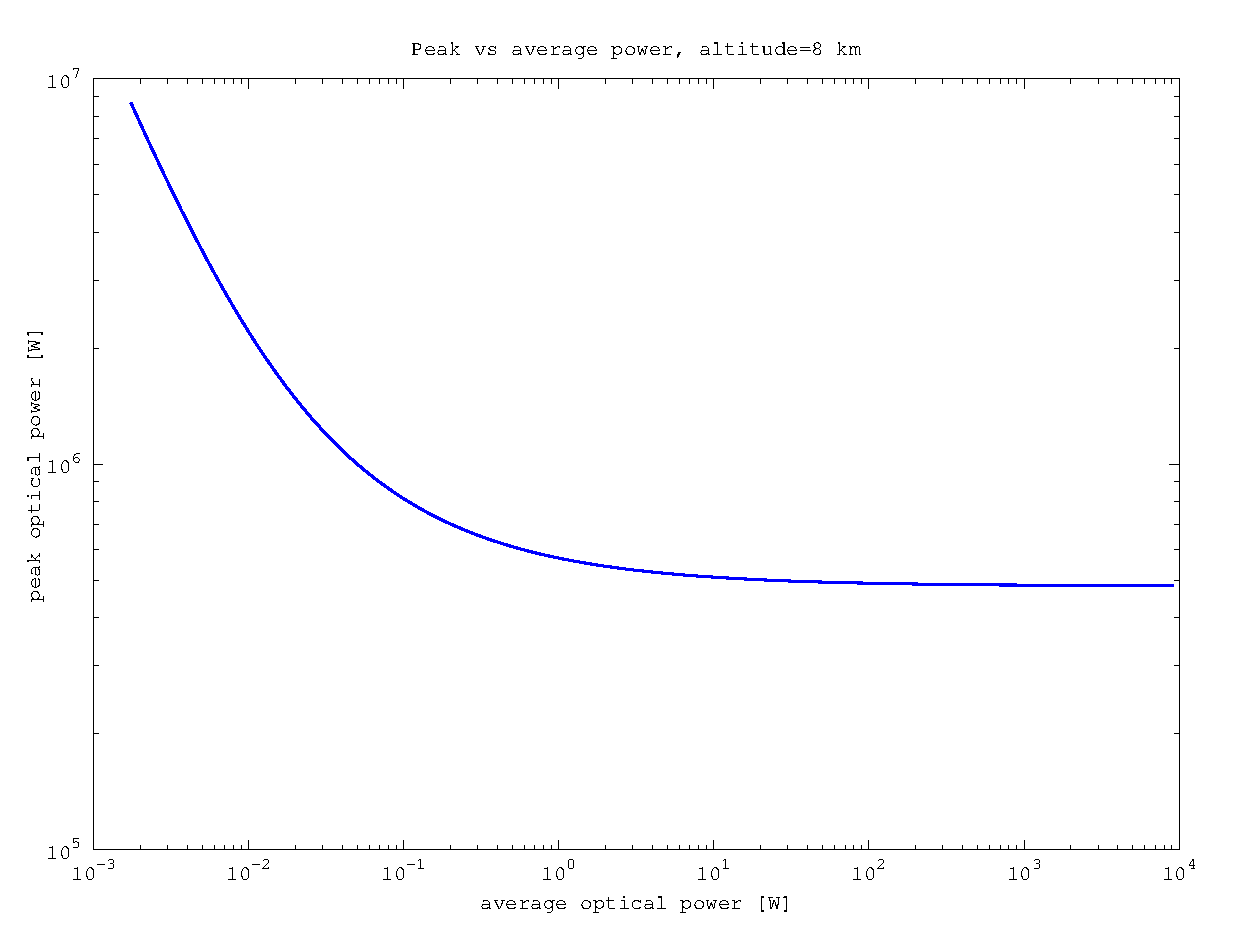
\includegraphics[width=0.8\linewidth]{fig/peak_vs_av.eps}
\caption{Relationship between number of signal and noise photons to get the required resolution}
\label{fig:temp_label}
\end{figure}

% \begin{figure}[h]
% \centering
% 	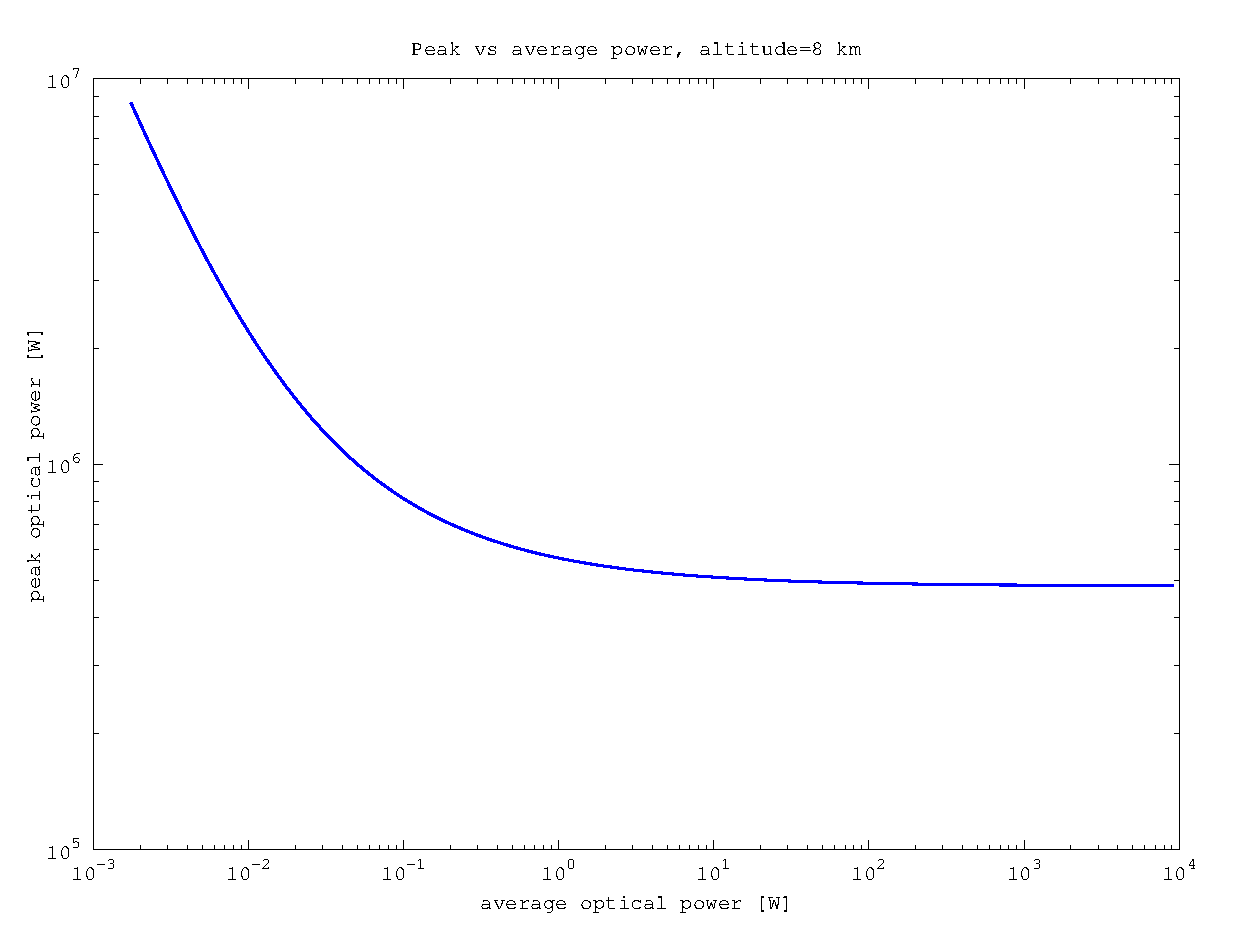
\includegraphics[width=0.8\linewidth]{fig/peak_vs_av.eps}
% \caption{required peak power for a given average power for the requirements at an altitude of $8\,km$}
% \label{fig:peak_vs_av}
% \end{figure}

When the energy threshold is added a very different relationship can be found. The threshold can be so powerful that noise can be almost completely eliminated without losing any signal photons, as long as the difference between the expected number of signal photons per bin is sufficiently larger than the expected number of noise photons per bin. To avoid pileup, it is assumed that a difference of a factor $F=4$ will be sufficient. It will also be assumed that a single pulse will be enough to acquire the required information. Using the calculations in \cref{tab:p_av_matching}, one can quickly tell that the peak optical power must be at least $1.9\,MW$. This is still an enourmous amount of peak power to produce, and hardly feasable.

\subsubsection{Reducing the field of view}
The limit calculated in \cref{tab:p_av_matching} is too high to design feasable laser specifications. The only way to reduce this lower limit, the amount of observed background noise must be further limited. To limit the amount of observed background noise, the field of view must be limited. Until this point the amount of background noise was defined as the amount of noise hitting the device from a $125\times125\,m^2$ surface on Europa at an altitude of $500\,m$. This means that on an altitude of $8\,km$, a surface of $2\times2\,km$ is obsverved. Now we take a look at what happens when the field of view is limited to a thin slice of $125\times0.1\,m^2$. Assuming that the laser is capable of tranmitting exactly into the small target area, this reduces the limit calculated in \cref{tab:p_av_matching} by a factor 1250. This shows that the altimetry mode for the laser is feasable, but that a sufficiently limited field of view is required. The target area for the Altimetry Mode can be arbitrarily small. The field of view can be limited by either the lens, or by disabling a portion of the SPADs on the chip.